\documentclass{article}

\usepackage{graphicx}

\begin{document}
\title{Homework 15}
\date{}
\maketitle

% 1. Fall 2009 Final, #4
% 2. Fall 2010 Final, #5
% 3. Textbook 4.3.1 and 4.4.1

\paragraph{\Large 1. Spring 2008 Final Questions 2a and 2b}\mbox{}\\
Run \textit{Dijkstra’s algorithm} on the weighted digraph below, starting at vertex $A$.\\
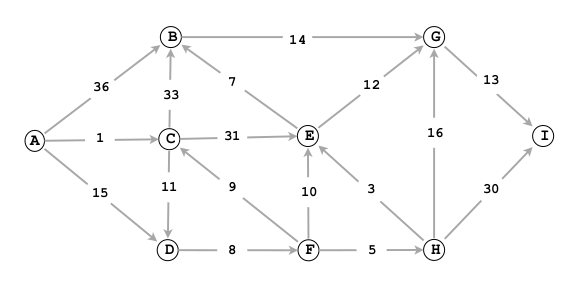
\includegraphics[]{fin-f09-4.png}\\
\begin{enumerate}
\renewcommand{\theenumi}{\Alph{enumi}}
	\item List the vertices in the order in which the vertices are dequeued (for the first time) from the priority queue and give the length of the shortest path from $A$.\\
	
	vertex: A C D F H E B G I\\

	distance: 0 1 12 20 25 28 34 40 43

	\item Draw the edges in the shortest path tree with thick lines in the figure above.\\

	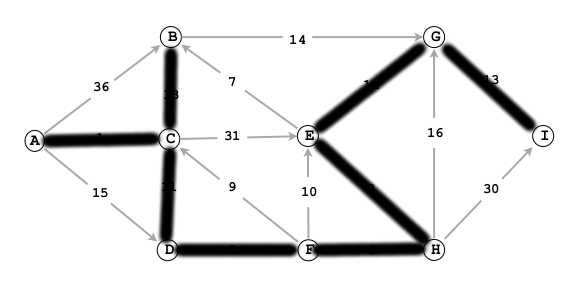
\includegraphics[]{fin-f09-4b.png}

\end{enumerate}


\paragraph{\Large 2. Fall 2010 Final Question 5}\mbox{}\\
Consider the following weighted graph with 10 vertices and 21 edges. Note that the edge weights are distinct integers between 1 and 21.\\
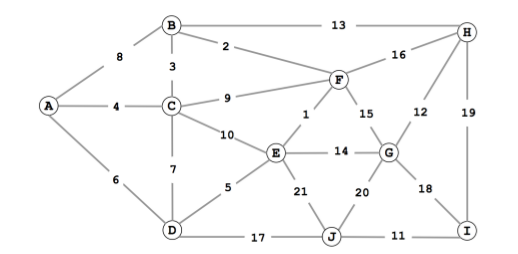
\includegraphics[]{fin-f08-2.png}\\
\begin{enumerate}
\renewcommand{\theenumi}{\Alph{enumi}}
	\item Complete the sequence of edges in the MST in the order that \textit{Kruskal's algorithm} includes them.\\

	1 2 3 4 5 11 12 13 17

	\item Complete the sequence of edges in the MST in the order that \textit{Prim's algorithm} includes them. Start Prim's algorithm from vertex $A$\\

	4 3 2 1 5 13 12 17 11
\end{enumerate}

\paragraph{\Large 3. Study Guide Question}\mbox{}\\
Would Kruskal's or Prim's algorithm work with edge-weighted digraphs?\\

No. It is possible to imagine a scenario in which the edge that either algorithm would pick could not be picked due to the direction of the graph's edges.

\end{document}